\section{Resultados}
En los sistemas biológicos las partículas se encuentran aleatoriamente orientadas, por lo que es conveniente calcular las secciones transversales promedio $\langle C_{abs}\rangle$ y $\langle C_{sca}\rangle$, que consideran que las partículas se iluminan con ondas electromagnéticas con polarización a lo largo de sus tres ejes principales de forma homogénea, \footnote{Considerando que las partículas no sean ópticamente activas.} éstas están dadas por \cite{Bohren}:
\begin{align*}
	\langle C_{abs}\rangle &= \frac{k}{3} \text{Im}\{\alpha^{(1)}+\alpha^{(2)}+\alpha^{(3)}\},\\
	\langle C_{sca}\rangle &= \frac{k^4}{3(6\pi)} \left(\alpha^{(1)}+\alpha^{(2)}+\alpha^{(3)}\right)^2.
\end{align*}

En este trabajo se calculan las secciones transversales promedio para elipsoides oblatos, empleados como una primera aproximación a la forma discoide cóncava de los eritrocitos. Debido a la simetría de estos elipsoides, las secciones transversales de extinción, absorción y esparcimiento producidas al aplicar un campo  polarizado en las direcciones $\hat{e}_x$ y $\hat{e}_y$ son iguales, es decir, $C_{ext}^{(1)}=C_{ext}^{(2)}$. Estas cantidades macroscópicas dependen directamente de la respuesta dieléctrica del material.\\

Para caracterizar la respuesta dieléctrica del material, se emplea la función dieléctrica $\epsilon(\omega)$, la cual puede determinarse experimentalmente a partir del índice de refracción complejo de un medio, $\tilde{n}(\omega) = n(\omega) + i\kappa(\omega)$. La relación entre la función dieléctrica y el índice de refracción está dada por las expresiones \cite{Plasmonics}
\begin{align} 
	\text{Re}[\epsilon(\omega)] &= n^2 - \kappa^2,\\
	\text{Im}[\epsilon(\omega)] &= 2n\kappa, \end{align}
donde $\kappa$ es el coeficiente de extinción, el cual describe la absorción de las ondas electromagnéticas al propagarse en el medio \cite{Plasmonics}.\\

En un determinado rango de frecuencias, las propiedades ópticas de los materiales pueden describirse mediante un modelo de plasma, en el cual un gas de electrones libres, con densidad numérica $n_e$, se mueve sobre un fondo fijo de núcleos de iones positivos \cite{Plasmonics}. Este enfoque, conocido como el modelo de Drude, es particularmente útil para describir el comportamiento dieléctrico de materiales en los que la respuesta óptica está dominada por electrones libres, como en los metales, donde los electrones en la banda de conducción responden colectivamente a un campo electromagnético aplicado. Mediante este modelo, se expresa a la función dieléctrica como \cite{Plasmonics}
\begin{equation} \epsilon(\omega) = 1 - \frac{\omega_p^2}{\omega^2 + i\gamma\omega}, \end{equation}
donde $\omega_p$ es la frecuencia de plasma del material y $\gamma$ es la constante fenomenológica de amortiguamiento. Debido a su dependencia exclusiva de la frecuencia, el modelo de Drude ofrece un mayor control sobre la respuesta óptica del sistema, por lo que resulta adecuado para realizar los cálculos iniciales y comprender su comportamiento.\\

Para analizar las contribuciones de las secciones transversales en partículas elipsoidales oblatas dentro del régimen cuasiestático, en la Fig. \ref{Contribuciones} se muestran las curvas de extinción (línea azul), esparcimiento (línea verde) y absorción promedio (línea roja), representadas por $\langle C_{ext} \rangle$, $\langle C_{sca} \rangle$ y $\langle C_{abs} \rangle$, respectivamente. Estas cantidades se grafican en escala logarítmica en función de la longitud de onda $\lambda$ y la energía $\hbar\omega$ de la onda electromagnética incidente. Las partículas elipsoidales oblatas son modeladas con una función dieléctrica dada por el modelo Drude, cuyos parámetros son $\hbar\omega_p=13.142\text{ eV}$ y $\hbar\gamma=0.197\text{ eV}$. Sus semiejes están dados por $a=b=1.5\text{ nm}$, $c=1\text{ nm}$ y se encuentra inmersa en una matriz con índice de refracción $n_m=1.33$. \\
\begin{figure}[h!]
	\sidesubfloat[]{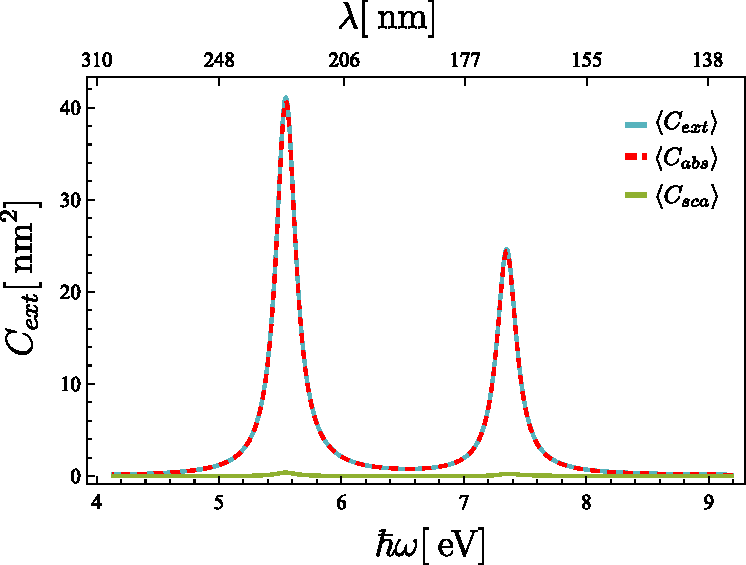
\includegraphics[width=.445\textwidth]{../../Figuras/AlContribuciones3.pdf} \label{Contribuciones}}\quad%
	\sidesubfloat[]{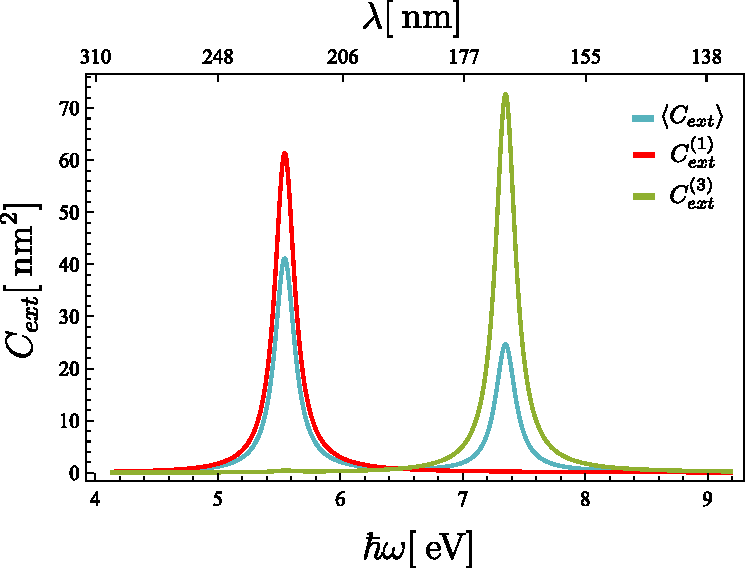
\includegraphics[width=.44\textwidth]{../../Figuras/CextAlbueno.pdf}\label{Cextpromedio}}%
	\caption{Secciones transversales como función de la energía $\hbar\omega$ y de la longitud de onda $\lambda$ para una partícula elipsoidal oblata de aluminio caracterizada por su función dieléctrica dada por el modelo de Drude ($\hbar\omega_p=13.142\text{ eV}$, $\hbar\gamma=0.197\text{ eV}$), con semiejes $a=b=1.5\text{ nm}$, $c=1\text{ nm}$ e inmersa en un medio acuoso ($n_m=1.33$). \textbf{a)}  Sección transversal de extinción promedio $\langle C_{ext}\rangle$  (línea azul), sección transversal de absorción promedio $\langle C_{abs}\rangle$  (línea roja) y sección transversal de esparcimiento promedio $\langle C_{sca}\rangle$  (línea verde) en escala logarítmica. \textbf{b)} Sección transversal de extinción promedio $\langle C_{ext}\rangle$ (línea azul), sección transversal de extinción al iluminar a la partícula con una onda polarizada en la dirección $\hat{e}_x$, $C_{ext}^{(1)}$  (línea roja)  y sección transversal de extinción al iluminar la partícula con una onda polarizada en la dirección $\hat{e}_z$ $C_{ext}^{(3)}$  (línea verde).} \label{fig:test}
\end{figure}

A partir de los resultados mostrados en la Fig. \ref{Contribuciones}, se observa que, en partículas dentro del régimen cuasiestático, la absorción domina sobre el esparcimiento en la contribución a la extinción. Esto se evidencia en la diferencia de magnitudes entre ambas curvas, donde la absorción es aproximadamente tres órdenes de magnitud mayor que el esparcimiento y la curva de extinción es escencialmente la misma que la de absorción. Debido a esta marcada diferencia, los análisis posteriores se enfocan exclusivamente en las secciones transversales de extinción, ya que el impacto del esparcimiento es despreciable.\\

El análisis de las diferencias entre la sección transversal de extinción promedio y aquellas obtenidas al iluminar la partícula con una onda polarizada en una única dirección alineada sobre los ejes principales se presenta en la Fig. \ref{Cextpromedio}. En esta figura se muestran las curvas de extinción promedio $\langle C_{ext}\rangle$ (línea azul), extinción para una onda polarizada en la dirección $\hat{e}_x$ ($C_{ext}^{(1)}$) (línea roja) y extinción para una onda polarizada en la dirección $\hat{e}_z$ ($C_{ext}^{(3)}$) (línea verde). Estos cálculos corresponden a un sistema con las mismas características que el de la Fig. \ref{Contribuciones}.\\

En la Fig. \ref{Cextpromedio} se observa que debido a la geometría de la partícula, que es un elipsoide oblato, la sección transversal de extinción promedio 
$\langle C_{ext}\rangle$ presenta dos máximos, los cuales coinciden con las frecuencias de los máximos de $C_{ext}^{(1)}$ y $C_{ext}^{(3)}$. Esto muestra que las secciones transversales promedio son útiles para representar el efecto de iluminar una partícula elipsoidal con una onda electromagnética polarizada en la dirección de cualquiera de sus tres ejes principales, ya que lo que cambia es la amplitud de los máximos en la sección transversal promedio más no la localización espectral de estos. \\

Las siguientes figuras presentan los cálculos de las secciones tranversales de extinción promedio  $\langle C_{ext}\rangle$ considerando nanopartículas elipsoidales oblatas cuya función dieléctrica está caracterizada por el modelo de Drude para aluminio \cite{Aluminio} y por datos experimentales para plata \cite{Plata}, oro \cite{Plata}, bismuto \cite{Bismuto} y  óxido de magnesio \cite{MgO}.


\subsection*{Aluminio y plata}
En la Fig. \ref{aluminioplataAR} se muestran las secciones transversales de extinción promedio $\langle C_{ext}\rangle$ en función de la energía $\hbar\omega$ y de la longitud de onda $\lambda$  de la onda electromagnética incidente en partículas elipsoidales oblatas de aluminio (Fig. \ref{aluminioAR}) y plata (Fig. \ref{plataAR}). La función dieléctrica para la partícula de plata está dada por el modelo de Drude con parámetros $\hbar\omega_p=13.142\text{ eV}$, $\hbar\gamma=0.197\text{ eV}$, mientras que para las partículas de aluminio la función dieléctrica está dada por datos experimentales obtenidos de \cite{Plata}. Se realizan los cálculos para partículas elipsoidales con semiejes de tamaños $a=2.5 \text{ nm}, c=1.25 \text{ nm}$ (línea azul), $a=2 \text{ nm}, c=1 \text{ nm}$ (línea verde), $a=1.5 \text{ nm}, c=0.75 \text{ nm}$ (línea naranja) y $a=1 \text{ nm}, c=0.5 \text{ nm}$ (línea roja) que presentan relaciones de aspecto  AR$=a/c=2$. Asimismo, se realizan los cálculos para una partícula esférica con tamaño $a=b=c=2 \text{ nm}$ (línea gris punteada) con relación de aspecto AR$=1$. Todas las partículas se consideran inmersas en un medio acuoso ($n_m=1.33$).\\

\begin{figure}[h!]
	\sidesubfloat[]{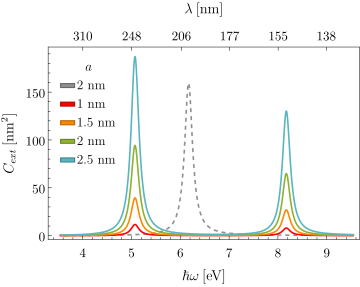
\includegraphics[width=.445\textwidth]{../../Figuras/AlAR} \label{aluminioAR}}\quad%
	\sidesubfloat[]{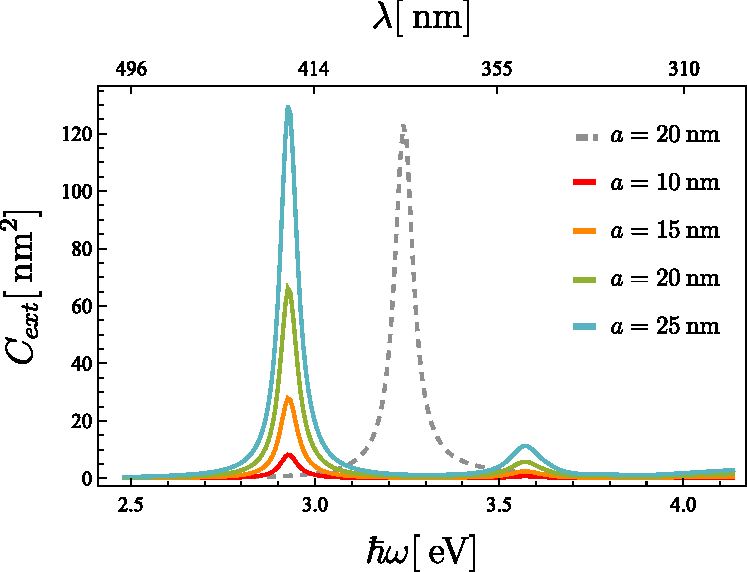
\includegraphics[width=.44\textwidth]{../../Figuras/AgAR}\label{plataAR}}%
	\caption{Secciones transversales de extinción promedio $\langle C_{ext}\rangle$ como función de la energía $\hbar\omega$ y de la longitud de onda $\lambda$ de la onda electromagnética incidente para una partícula elipsoidal oblata con razón de aspecto $AR=a/c=2$ constante, excepto en el caso de una esfera (línea gris punteada) donde $AR=1$. Las partículas poseen semiejes de tamaños $a=2.5 \text{ nm}, c=1.25 \text{ nm}$ (línea azul), $a=2 \text{ nm}, c=1 \text{ nm}$ (línea verde), $a=1.5 \text{ nm}, c=0.75 \text{ nm}$ (línea naranja), $a=1 \text{ nm}, c=0.5 \text{ nm}$ (línea roja) y $a=b=c=2\text{ nm}$ (línea gris punteada). Las partículas se encuentran inmersas en un medio acuoso ($n_m=1.33$) y están caracterizadas por su función dieléctrica dada por  \textbf{a)} el modelo de Drude para el aluminio con parámetros $\hbar\omega_p=13.142\text{ eV}$ y $\hbar\gamma=0.197\text{ eV}$) y \textbf{b)} datos experimentales correspondientes a la plata obtenidos de \cite{Plata}. }\label{aluminioplataAR}
\end{figure}
A partir de los resultados de la Fig. \ref{aluminioplataAR}, se observa que al aumentar el tamaño de la partícula mientras se mantiene constante la relación de aspecto, la localización espectral de las resonancias no cambia pero que su amplitud aumenta. Se identifican dos máximos locales en la sección de transversal extinción promedio,  los cuales corresponden a las frecuencias en las que la extinción se maximiza al iluminar la partícula en las direcciones $\hat{e}_x$ y $\hat{e}_z$. En la dirección $\hat{e}_x$, las resonancias  se encuentran en $\lambda=$254 nm para el aluminio y $\lambda=$434 nm para la plata. En la dirección $\hat{e}_z$, las resonancias ocurren en $\lambda=$146 nm para aluminio y $\lambda=$344 nm para la plata. \\

El efecto de la variación de la relación de aspecto en la sección transversal de extinción promedio en partículas de aluminio y plata inmersas en un medio acuoso ($n_m=1.33$) se muestra en la Fig. \ref{aluminioplatac}. Se muestra la sección transversal promedio $\langle C_{ext}\rangle$ en función de la energía $\hbar\omega$ y de la longitud de onda $\lambda$  de la onda electromagnética incidente en partículas elipsoidales oblatas de aluminio (Fig. \ref{aluminioc}) y plata (Fig. \ref{platac}). Las funciones dieléctricas utilizadas para las partículas de aluminio y las de plata son las mismas que en la Fig. \ref{aluminioplataAR}. Se realizan los cálculos para partículas elipsoidales con razones de aspecto AR=1.5 (línea roja), AR=1.75 (línea naranja), AR=2 (línea verde) y AR=2.25 (línea azul) que presentan valores en su semieje mejor $c=1\text{ nm}$. Asimismo, se realizan los cálculos para una partícula esférica con semieje mejor $c=1\text{ nm}$ y con relación de aspecto AR$=1$. 


\begin{figure}[h!]
	\sidesubfloat[]{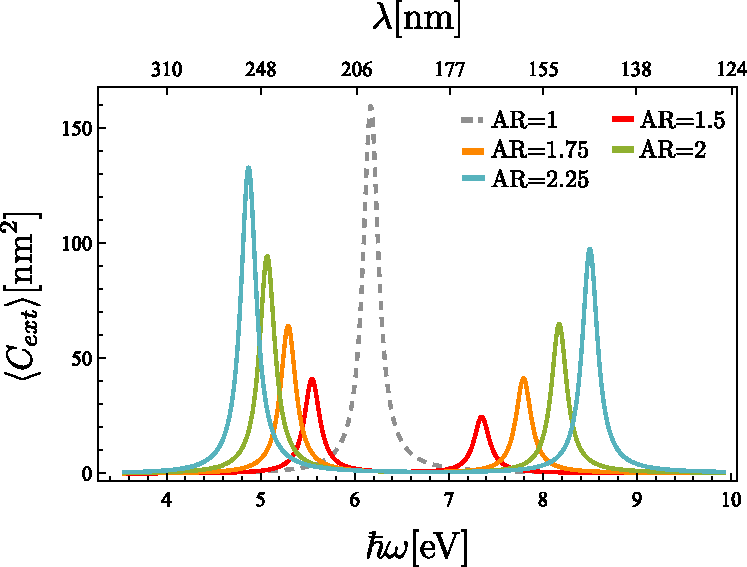
\includegraphics[width=.445\textwidth]{../../Figuras/Alc} \label{aluminioc}}\quad%
	\sidesubfloat[]{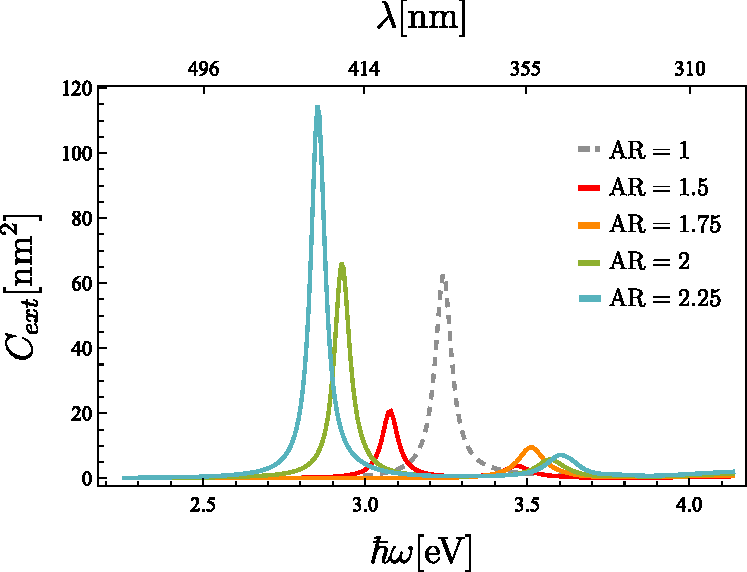
\includegraphics[width=.44\textwidth]{../../Figuras/Agc}\label{platac}}%
	\caption{Secciones transversales de extinción promedio $\langle C_{ext}\rangle$ como función de la energía $\hbar\omega$ y de la longitud de onda $\lambda$ de la onda electromagnética incidente para una partícula elipsoidal oblata y una esférica. Las partículas elipsoidales poseen un semieje menor de tamaño $c=1nm$ y presentan razones de aspecto de AR=1.5 (línea roja), AR=1.75 (línea naranja), AR=2 (línea verde), AR=2.25 (línea azul), mientras que la esférica tiene una razón de aspecto AR=1 (línea gris punteada). Las partículas están inmersas en un medio acuoso ($n_m=1.33$) y están caracterizadas por su función dieléctrica dada por  \textbf{a)} el modelo de Drude para el aluminio ($\hbar\omega_p=13.142\text{ eV}$, $\hbar\gamma=0.197\text{ eV}$) y \textbf{b)} datos experimentales correspondientes a la plata obtenidos de \cite{Plata}.}\label{aluminioplatac}
\end{figure} 

 En las Figs. \ref{aluminioc}  y \ref{platac} se observa que conforme la relación de aspecto se aproxima a la unidad, hay un corrimiento de las frecuencias asociadas a las $\langle C_{ext}\rangle$ máximas hacia la frecuencia de resonancia asociada a una partícula esférica. Esta frecuencia de resonancia corresponde a $\lambda=201\text{ nm}$ para el aluminio y $\lambda=383\text{ nm}$ para la plata. Además, tanto en el aluminio como en la plata, se observa que al aumentar la relación de aspecto y la longitud del eje mayor, la amplitud de  $\langle C_{ext}\rangle$ también aumenta. Esto se debe a que una mayor sección transversal efectiva de interacción con la onda electromagnética incrementa la probabilidad de esparcimiento y absorción de luz, lo que, en consecuencia, aumenta la extinción.



\subsection*{Oro y bismuto}

La Fig. \ref{oro} muestra el análisis del efecto de la variación de la razón de aspecto en las secciones transversales de extinción de partículas elipsoidales oblatas de oro. Se observan las secciones transversales de extinción promedio  $\langle C_{ext}\rangle$ para partículas de oro, así como la parte imaginaria (línea azul) y real (línea roja) de su función dieléctrica como función de la energía $\hbar\omega$ y de la longitud de onda $\lambda$ de la onda electromagnética incidente. En la Fig. \ref{oroAR} se consideran partículas con relación de aspecto AR$=2$ con tamaños de semiejes $a=2.5 \text{ nm}, c=1.25 \text{ nm}$ (línea azul), $a=2 \text{ nm}, c=1 \text{ nm}$ (línea verde), $a=1.5 \text{ nm}, c=0.75 \text{ nm}$ (línea naranja) y $a=1 \text{ nm}, c=0.5 \text{ nm}$ (línea roja). También se considera una partícula con relación de aspecto AR$=1$ y semiejes $a=b=c=2$ nm (línea gris), que representa a una partícula esférica. Por otro lado, en la Fig. \ref{oroc} se consideraron partículas con relación de aspecto variable AR=1.5 (línea roja), AR=1.75 (línea naranja), AR=2 (línea verde) y AR=2.25 (línea azul) que presentan valores en su semieje menor $c=1\text{ nm}$. Asimismo, se considera una partícula esférica con semieje mejor $c=1\text{ nm}$ y con relación de aspecto AR$=1$ (línea gris).
\begin{figure}[H]
	\sidesubfloat[]{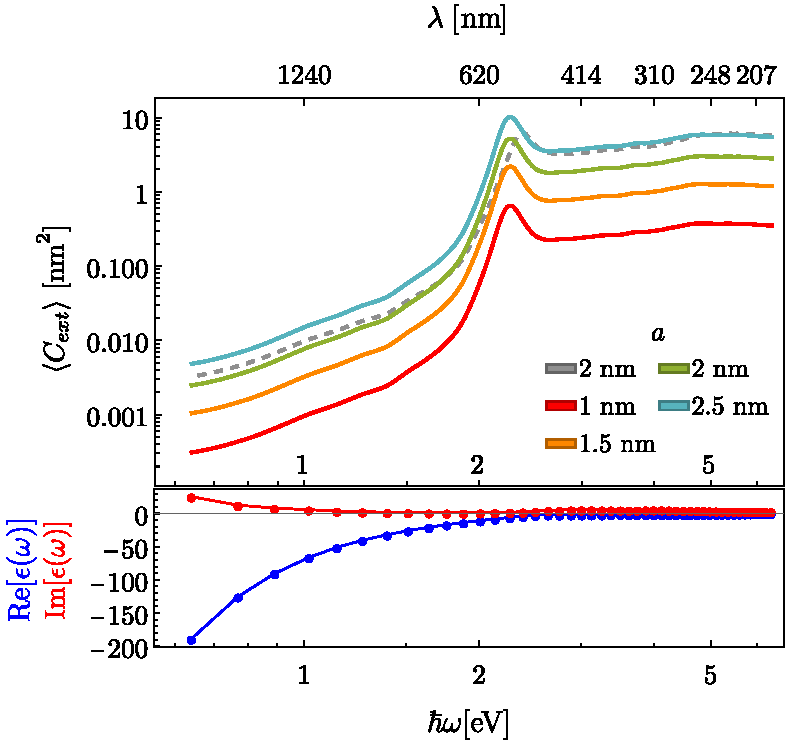
\includegraphics[width=.445\textwidth]{../../Figuras/Au2.pdf} \label{oroAR}}\quad%
	\sidesubfloat[]{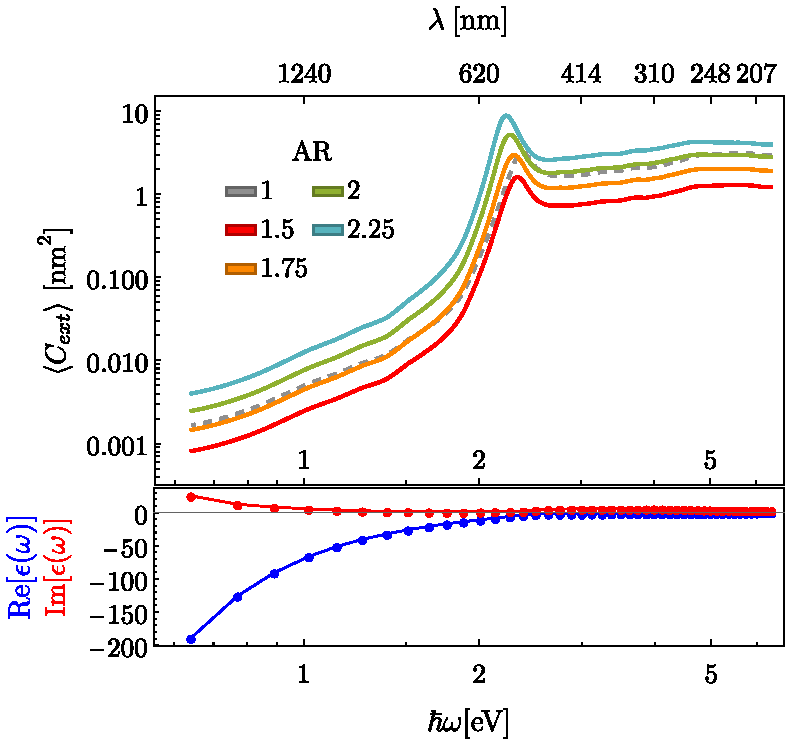
\includegraphics[width=.44\textwidth]{../../Figuras/Au.pdf}\label{oroc}}%
	\caption{Secciones transversales de extinción promedio $\langle C_{ext}\rangle$ como función de la energía $\hbar\omega$ y de la longitud de onda $\lambda$ para una partícula elipsoidal oblata de oro, cuyo índice de refracción complejo fue obtenido a partir de datos experimentales  e inmersa en agua ($n_m=1.33$) y curvas de comparación del índice de refracción (parte real en azul, parte imaginaria en rojo) como función de la energía $\hbar\omega$ y de la longitud de onda $\lambda$ para el oro. \textbf{a)} Razón de aspecto $AR=2$ constante, excepto en el caso de una esfera (línea gris punteada) donde $AR=1$. \textbf{b)} Semieje menor $c=1$ nm constante.}\label{oro}
\end{figure}

En contraste con el aluminio y la plata, en la Fig. \ref{oro} se observa solo una frecuencia de resonancia en $\lambda=$ 547 nm, que se atribuye a la fuerte absorción del oro en el espectro visible, lo que suprime resonancias adicionales. El aumento de la sección transversal de extinción se debe a que para energías mayores a 1.76 eV, los electrones ligados empiezan a contribuir significativamente por medio de transiciones interbanda. Se observa que conforme la relación de aspecto se aproxima a la unidad, hay un corrimiento de las frecuencias asociadas a las $\langle C_{ext}\rangle$ máximas hacia una frecuencia de resonancia ($557\text{ nm}$) asociada a una esfera de oro inmersa en agua. 



En la Fig. \ref{bismuto} se observan las secciones transversales de extinción promedio para partículas de bismuto, así como la parte imaginaria y real de su índice de refracción. En la Fig. \ref{bismutoAR} se consideraron partículas con relación de aspecto AR$=2$  y en la Fig. \ref{bismutoc} se consideraron partículas con relación de aspecto variable. En ambas figuras es posible observar una frecuencia de resonancia de alrededor de los 154 nm.

\begin{figure}[H]
	\sidesubfloat[]{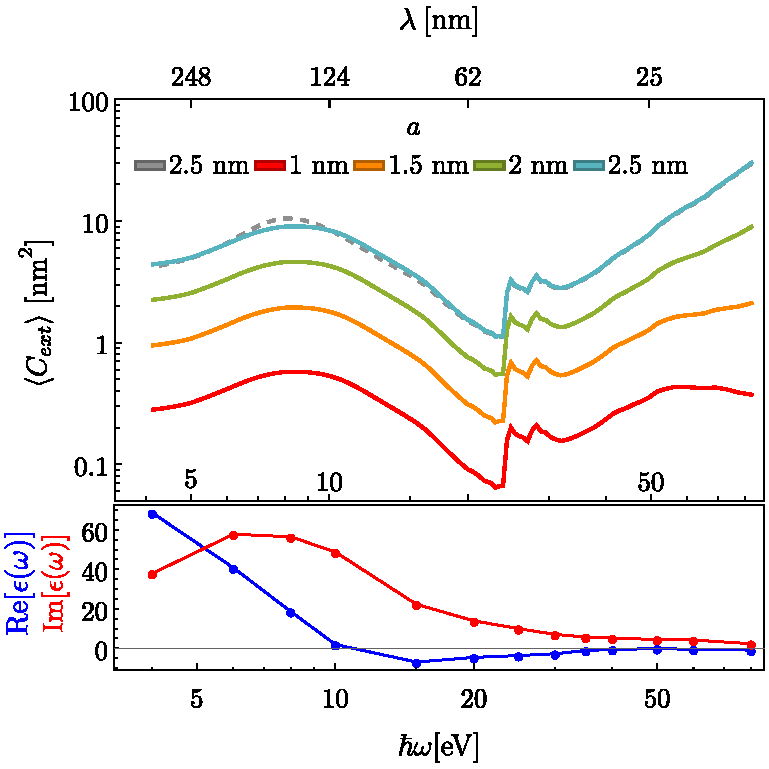
\includegraphics[width=.445\textwidth]{../../Figuras/Bi2} \label{bismutoAR}}\quad%
	\sidesubfloat[]{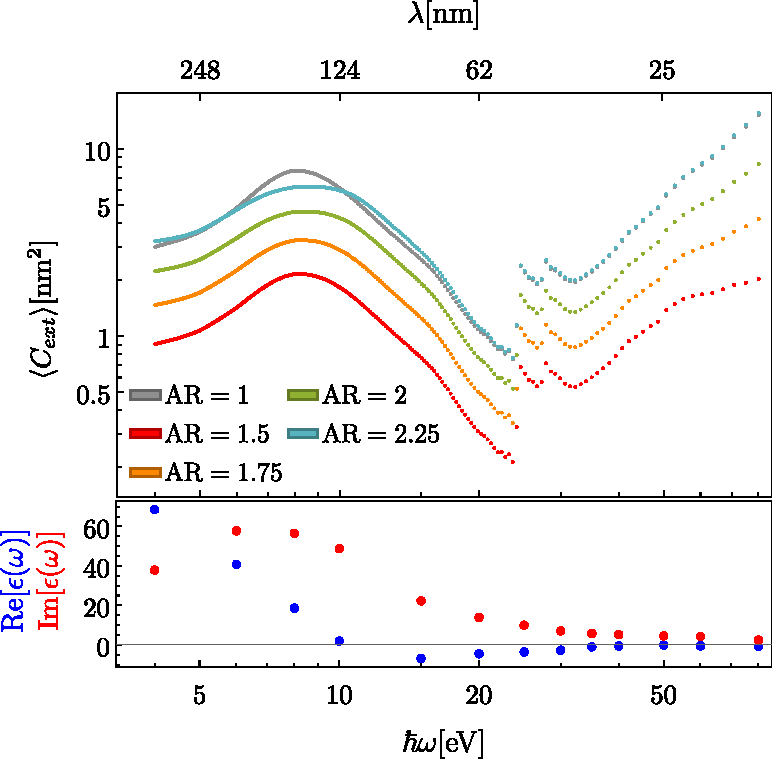
\includegraphics[width=.44\textwidth]{../../Figuras/Bi}\label{bismutoc}}%
	\caption{Secciones transversales de extinción promedio $\langle C_{ext}\rangle$ como función de la energía $\hbar\omega$ y de la longitud de onda $\lambda$ para una partícula elipsoidal oblata de bismuto, cuyo índice de refracción complejo fue obtenido a partir de datos experimentales  e inmersa en agua ($n_m=1.33$) y curvas de comparación de la función dieléctrica (parte real en azul, parte imaginaria en rojo) como función de la energía $\hbar\omega$ y de la longitud de onda $\lambda$ para el bismuto. \textbf{a)} Razón de aspecto $AR=2$ constante, excepto en el caso de una esfera (línea gris punteada) donde $AR=1$. \textbf{b)} Semieje menor $c=1$ nm constante.}\label{bismuto}
\end{figure}


\subsection*{Óxido de magnesio}
En la Fig. \ref{mgo} se observan las secciones transversales de extinción promedio para partículas de bismuto, así como la parte imaginaria y real de su índice de refracción. En la Fig. \ref{mgoAR} se consideraron partículas con relación de aspecto AR$=2$  y en la Fig. \ref{mgoc} se consideraron partículas con relación de aspecto variable. En ambos casos se observa que la $\langle C_{ext}\rangle$ tiene un comportamiento creciente pues, dado que en el espectro de las ondas de radio, la contribución de la absorción es nula y la única contribución es la del esparcimiento, que aumenta al disminuir la longitud de onda.

\begin{figure}[H]
	\sidesubfloat[]{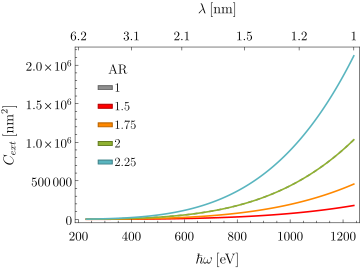
\includegraphics[width=.445\textwidth]{../../Figuras/MgOc} \label{mgoc}}\quad%
	\sidesubfloat[]{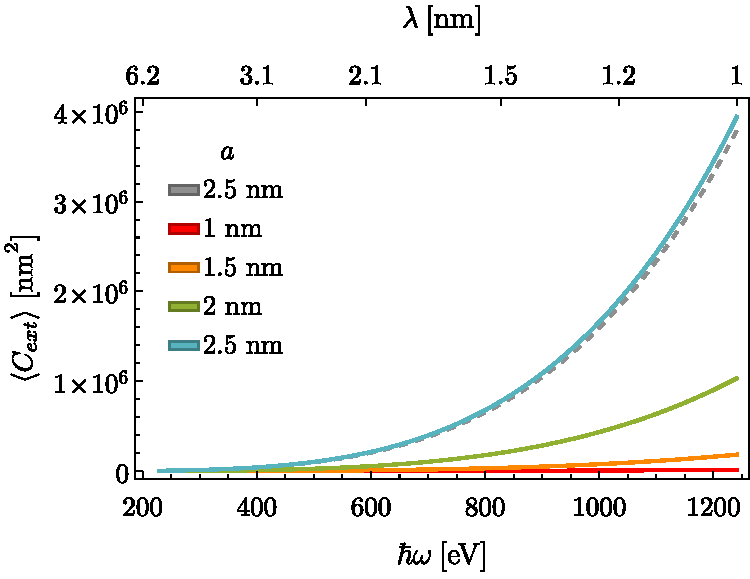
\includegraphics[width=.44\textwidth]{../../Figuras/MgOAR}\label{mgoAR}}%
	\caption{Secciones transversales de extinción promedio $\langle C_{ext}\rangle$ como función de la energía $\hbar\omega$ y de la longitud de onda $\lambda$ para una partícula elipsoidal oblata de óxido de magnesio, cuyo índice de refracción complejo fue obtenido a partir de datos experimentales  e inmersa en agua ($n_m=1.33$) y curvas de comparación de la función dieléctrica (parte real en azul, parte imaginaria en rojo) como función de la energía $\hbar\omega$ y de la longitud de onda $\lambda$ para el bismuto. \textbf{a)} Razón de aspecto $AR=2$ constante, excepto en el caso de una esfera (línea gris punteada) donde $AR=1$. \textbf{b)} Semieje menor $c=1$ nm constante.}\label{mgo}
\end{figure}

Tiene transiciones interbanda a energías muy bajas (~0.15 - 0.2 eV, en el infrarrojo medio).
Se comporta como un semimetal, con una densidad de estados electrónica muy baja en el nivel de Fermi.
En el visible y el infrarrojo cercano, su respuesta óptica es más compleja y no sigue el modelo simple de plasma.







